\documentclass[11pt]{article}
\usepackage{natbib}
\usepackage{float}
\usepackage[pdftex]{graphicx}     % could insert ``draft'' between []
\usepackage{amsmath}
\pagestyle{empty}
\setlength{\oddsidemargin}{0pt}
\setlength{\textwidth}{6.5in}
\setlength{\voffset}{0pt}
\setlength{\topmargin}{-0.75in}
\setlength{\textheight}{10.0in}
%%%%%%%%%%%

\newcommand{\kvec}{{\bf k}}
\newcommand{\bvec}{{\bf b}}
\newcommand{\shat}{{\hat s}}
\newcommand{\kpr}{{k_\perp}}
\newcommand{\kvpr}{{\kvec_\perp}}
\newcommand{\kpl}{{k_\parallel}}
\newcommand{\AI}{{\langle\tilde A*\tilde I\rangle}}
\newcommand{\AItau}{{\AI(\tau)}}
\newcommand{\hMpci}{{h~{\rm Mpc}^{-1}}}
\newcommand{\lsim}{{<\sim}} % XXX put real command here
\newcommand{\inch}{$^{\prime\prime}$}
\newcommand{\foot}{$^{\prime}$}
\renewcommand{\deg}{^\circ}

\begin{document}
\title{Diameter of the HERA Antenna}
\author{David DeBoer and Aaron Parsons}
\maketitle

\section{Introduction}

The design of the HERA element is driven by advances in our understanding of how
an interferometer's chromatic response interacts with foreground emission to
produce systematics in power spectral measurements of the 21cm reionization signal.

\section{Understanding Instrumental Chromaticity in the Context of the Wedge}

For this discussion, we average the three-dimensional power spectrum $P(\kvec)$ along a cylinder
of $k_x^2+k_y^2=\kpr^2$, where $\kvec\equiv(k_x,k_y,\kpl)$ is the three-dimensional wavevector,
$(k_x,k_y)$ are taken to be in the plane of the sky, and $\kpl$ is measured along the line-of-sight (spectral)
direction.
Recent work has shown that, for an interferometer whose
analog bandpass and beam chromaticity are sufficiently smooth, systematics arising from foreground emission
are isolated in the cylindrically averaged power spectrum $P(\kpr,\kpl)$ within
a wedge-shaped region described by \citep{parsons_et_al2012b,pober_et_al2013,parsons_et_al2014,ali_et_al2015}:
% XXX add the whole list of wedge cites
\begin{align}
|\kpl| &\le \frac{Y}{X\nu}\kpr + YS\nonumber\\
&\le \frac{Y}{c}b + YS,
\label{eq:wedge_bound}
\end{align}
where $X,Y$ are cosmological scalars relating angular size and spectral frequency to comoving 
physical size, respectively, $\nu$ is spectral frequency, and $b=|\bvec|$ is the magnitude of the baseline vector for
antennas in an interferometric pair, which substitutes for $\kpr$ according to the
relation $\kvpr=X\nu\bvec/c$. As we will derive below, $S$ is an additional additive offset related to
the combined spectral smoothness of foregrounds and the antenna response.

As pointed out in \citet{parsons_et_al2012b}, the factor of $b/c$ in the
second line of equation (\ref{eq:wedge_bound}) can be interpreted as the light-crossing time
or maximum geometric signal delay, $\tau_{b,max}$ associated with an interferometric baseline.  
Particularly for per-baseline
analyses such as those
employed on PAPER \citep{parsons_et_al2014,jacobs_et_al2015,moore_et_al2015,ali_et_al2015},
{\it signal delay} turns out to be a 
powerful basis for understanding the chromatic effects of interferometric observations.
Signal delay arises as the Fourier dual to spectral frequency, according to the delay
transformation of a visibility,
\begin{equation}
\tilde V_\bvec(\tau)=\int{d\nu~V_\bvec(\nu) e^{2\pi i\tau\nu}}.
\end{equation}
The measurement equation defines the visibility as
\begin{equation}
V_\bvec(\nu)=\int{d\Omega~A(\shat,\nu)~I(\shat,\nu) e^{-2\pi i\frac{\bvec\cdot\shat}{c}\nu}},
\label{eq:meas_eq}
\end{equation}
where $A$ is the antenna response as a function of directon $\shat$ and $I$ is the sky intensity.
We define the geometric signal delay in direction $\shat$ as $\tau_{\bvec,\shat}\equiv\bvec\cdot\shat/c$
in order to re-express the delay-transformed visibility as
\begin{align}
\tilde V_\bvec(\tau)&=\int\!\!\int{d\nu~d\Omega~A(\shat,\nu)~I(\shat,\nu) e^{-2\pi i\nu(\tau_{\bvec,\shat}-\tau)}}\nonumber\\
&=\int{d\Omega~\tilde A(\shat,\tau)*\tilde I(\shat,\tau)*\delta_D(\tau_{\bvec,\shat}-\tau)},
\end{align}
where $\delta_D$ is the Dirac delta function, `$~\tilde{}~$' signifies Fourier transformation along
the frequency axis, and `$*$' denotes convolution.

Under the ``delay approximation" \citep{parsons_et_al2012b},
signal delay $\tau$ can be interpreted as a reasonable approximation to $\kpl$, giving us the following relationship
between the delay-transformed visibility and the power spectrum:
\begin{equation}
\tilde V_\bvec^2(\tau)\approx\left(\frac{2k_B}{\lambda^2}\right)^2\frac{\Omega B}{X^2Y}\widehat P(\kvpr,\kpl),
\label{eq:v2_to_pk}
\end{equation}
where $k_B$ is Boltzmann's constant, $\lambda$ is spectral wavelength, $\Omega$ is the angular area of the power-squared
beam \citep{parsons_et_al2014}, and $B$ is the effective bandwidth over which the delay transformation is performed.

We can now revisit the bound on systematics arising from the interaction of foreground emission and
instrumental chromaticism given in equation (\ref{eq:wedge_bound}).  Let us assume for a moment that
$A$ and $I$ are perfectly flat functions of frequency, so that $\tilde A$ and $\tilde I$ are delta functions
centered at $\tau=0$.  In this case, the value of $\tilde V_\bvec(\tau)$ is determined by
the integral over $\tilde A(\shat,0)~\tilde I(\shat,0)$ in the sky directions that satisfy $\tau_{\bvec,\shat}=\tau$.
For a given baseline $\bvec=\kvpr/X\nu$, $\tau_{\bvec,\shat}$ is bounded by $\tau_{b,max}=b/c$, implying that
for the case we have outlined, $\tilde V_\bvec(\tau)$ must be zero outside of a region
$|\tau|\le b/c$.  Under the delay approximation, $\kpl\approx Y\tau$, so we can use equation
(\ref{eq:v2_to_pk}) say that $P(\kpr,\kpl)$ must be zero outside of the region specified in 
equation (\ref{eq:wedge_bound}) for $S=0$.

The inclusion of $S$ in equation (\ref{eq:wedge_bound}) accounts for precisely the terms we neglected above:
the spectral structure in $A$ and $I$, or more precisely, the delay-domain width of 
\begin{equation}
\AItau\equiv\int{d\Omega~\tilde A(\shat,\tau)*\tilde I(\shat,\tau)},
\end{equation}
where $\langle\dots\rangle$ denotes the average over solid angle.
In order to determine $S$ quantitatively, however,
we must clarify what is the relevant width in delay-domain.  The purpose of equation (\ref{eq:wedge_bound}) is 
to illustrate
the boundary between the systematics-dominated and signal-dominated regimes.
As such, it makes the most sense to determine width by the interval in
delay domain outside of which $\AItau$ is below the expected level
of the 21cm reionization signal.  Spectrally smooth ($\tau\approx0$) foregrounds are approximately
four to five times brighter that the expected reionization signal \citep{}, so a conservative definition of
$S$ requires
\begin{equation}
\frac{|\AItau|}{|\langle\tilde I\rangle(\tau=0)|}<10^{-6}.
\label{eq:def_S}
\end{equation}
In words, we define $S$ as the delay interval over which
$\AI$ falls off by -60 dB.

Given this framework, an obvious design goal for an interferometer aiming to 
measure the 21cm reionization signal is create antennas that can be close-packed to minimize $b$, and
which yield an antenna response that minimizes $S$.  However, as we will explore in more detail below, 
these aims must be balanced against cost.

% sky averaged 
\subsection{Inherent Chromaticity of Foregrounds}

Before we explore antenna design, however, it would be convenient to set an upper bound on the contribution of
$\tilde I$ in equation (\ref{eq:def_S}).  XXX this is turning out to be a bit tricky.  Result is strongly
dependent on windowing.  Choosing a Blackman-Harris window and playing with power-law spectral indices of
-1 and -2, getting a width for $\tilde I$ in range of 10 to 60 ns.

Suggest diminishing returns associated with pushing instrumental chromaticity much lower than 10 to 60 ns.

Also, as we push antennas closer together, galactic synchrotron emission (our dominant foreground) gets
brighter as $C_\ell\propto\ell^{-3}$ \citep{}.
Under the assumption that $\kpl$ is the dominant component of $\kvec$ (which
holds for the short baselines used in PAPER and HERA),
this implies that $|\AItau|^2$ must decrease more rapidly than $\tau^{-3}$ for a reduction in baseline length
to result in a reduction in foreground contamination at a given $\kpl$ scale.  Hence, the combined chromaticity
of the antenna beam and the galactic synchrotron foreground set an effective minimum baseline length, shorter
than which foreground systematics no longer decrease, and could even potientially extend further in $|\kpl|$.  
This departure from the
strictly linear relationship in equation (\ref{eq:wedge_bound}) (which we will call the ``ankle")
for the shortest baselines is a telltale sign
of the influence of diffuse synchrotron emission.

XXX If get analytic derivation of foreground profile in delay working, relate to that here.
Figure XXX in \citet{pober_et_al2013}
shows evidence of the departure equation (\ref{eq:wedge_bound}) described above for baselines shorter than
$\lsim10$ wavelengths.  Although this empirical result includes a contribution from the PAPER antenna beam,
the constant additive term that $\tilde A$ contributes (XXX maybe should capture in eq 1 that I could be baseline-dep)
to the wedge boundary does not change the position of the ankle.  Also worth noting is that, although an ankle
appears around $\sim9$ wavelengths, the extent of the wedge in $\kpl$ continues to decrease slowly toward 
even shorter baselines.  This implies that, while there are diminishing returns in foreground systematics for using
baseline shorter than $\sim18$ m (9 wavelengths at 150 MHz), there does not appear to be a strong penalty 
for doing so either.

\subsection{Setting an Antenna Specification}

So far, we have largely ignored the contribution of the antenna term in $\AItau$.  We now have
a handle on the chromaticism introduced by the baseline term in equation (\ref{eq:meas_eq}) and 
an indication of when shorter baselines stop linearly reducing the occupancy of
foreground systematics in $|\kpl|$.  As we argued above, $b\lsim20$ m is an approximate threshold
for when the chromaticity of the baseline term is no longer dominant.  This suggests that
foreground systematics are unlikely to drop below a width in delay domain corresponding to 
$b/c\sim60$ ns ($|\kpl|\sim0.03\hMpci$ at 150 MHz).

Therefore, a reasonable specification 
for an interferometer targeting 21cm power spectrum measurements and working outside
the wedge to avoid foregrounds might be to equally partition a chromaticity budget (i.e. delay-domain
width) between the baseline term $\delta_D(\tau_{\bvec,\shat}-\tau)$, 
the inherent foreground term $\tilde I(\shat,\tau)$, and the antenna term $\tilde A(\shat,\tau)$.
As described in equation (\ref{eq:def_S}), the relevant delay domain width 
is measured at the -60 dB point.  Therefore, the specification we set for the chromaticity
of the antenna is
\begin{equation}
\frac{|\langle\tilde A\rangle(\shat,\tau=60~{\rm ns})|}{|\tilde \langle A\rangle(\shat,\tau=0~{\rm ns})|}<10^{-6}.
\end{equation}
Here, we have separated the antenna and sky terms in $\AItau$ in order to set a specification for
the antenna term alone.

Under this specification, we assume the final chromaticity (wedge width) to be the sum of the
individual widths of the $\tilde A$, $\tilde I$, and $\delta_D(\tau_{\bvec,\shat}-\tau)$ terms,
for a total of 180 ns ($|\kpl|=0.9\hMpci$ at 150 MHz).


\section{HERA Antenna Design}

The diameter of the HERA antenna is set by three factors:  
%\begin{enumerate}
(1) meeting the delay reflection specification of 60 dB at 60 ns, (2) lessening the impact of systematics, (3) lessening cost for a fixed sensitivity.

\section{Delay}
The delay-delayrate analysis technique employed for HERA requires that the region of phase space employed has contamination below the level of the signal.  The supplied value from the analysis team is that reflections must be reduced by at least 60 dB at 60 ns.  Another formulation is VSWR $<$ 1.002 at frequencies below 15 MHz.  The reflections between the feed and vertex is a chief contributor.  The determine the delay scale a focal ratio must be used.  A series of analytical models was run at several diameters using the calculated beam pattern of the PAPER feed.  The results are shown in Figure \ref{fig:efficiency}.  Note that they all peak at about a focal ratio of 0.32 (the solid lines with the x-axis divided by 10).

\begin{figure}[h]
\centering
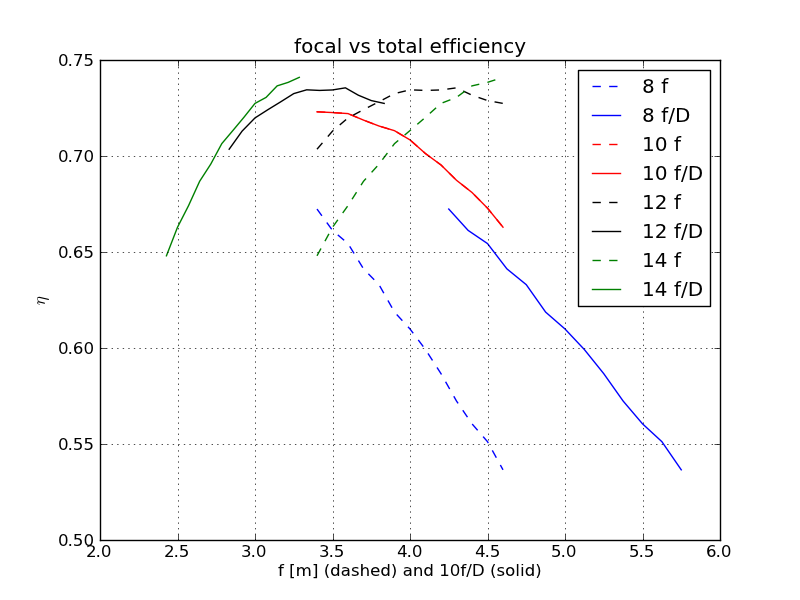
\includegraphics[width=0.8\textwidth]{heraDishfDplot.png}
\caption{Efficiencies of various diameters and focal lengths in one confusing plot.}
\label{fig:efficiency}
\end{figure}

Using an $f/D=0.32$, one can compute the round-trip times between the vertex and feed.  Figure \ref{fig:roundtrip} shows the round-trip ({\em i.e.} delay) times for 1, 2 and 3 trips with a vertical line at 60 ns, the delay spec.  This may be interpreted that for diameters of about 28-m you have one round-trip in which to attenuate by 60 dB, for a diameter of about 14-m  you have two round-trips and for diameters of about 9.4-m you have three round-trips. 
\begin{figure}[h]
\centering
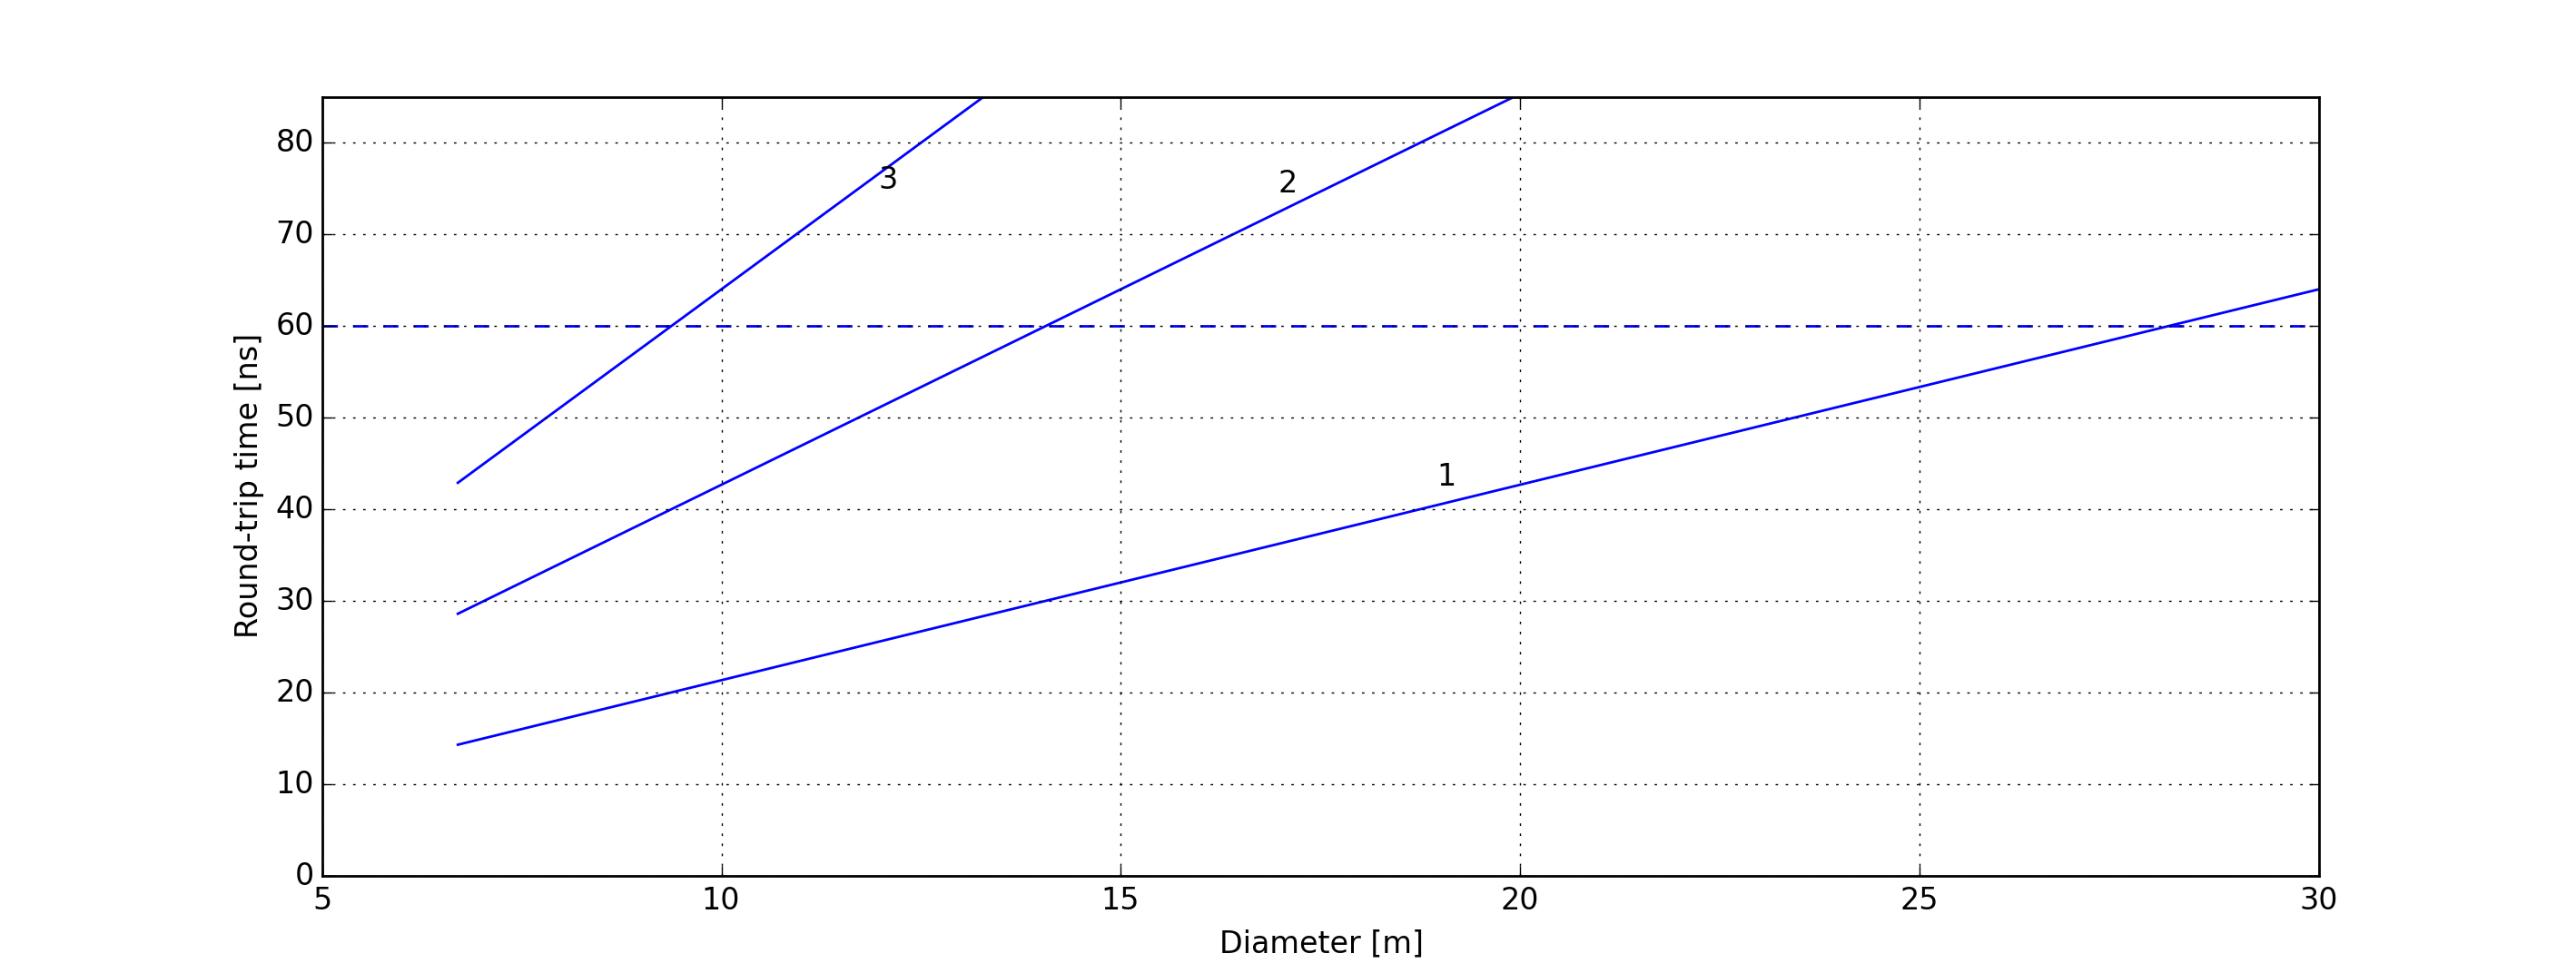
\includegraphics[width=1.0\textwidth]{roundtrip.png}
\caption{Round-trip times for $f/D=0.32$ for 1, 2 and 3 trips.}
\label{fig:roundtrip}
\end{figure}

If we assume an "attenuation/bounce" that takes into account the loss factors at each segment of the round-trip journeys (reflections, path loss, etc -- so we could have partial round-trips) we can look over a plausible range and see if they might feasibly provide enough overall attenuation.  Figure \ref{fig:bounces} plots this for 1, 2 and 3 round-trips.
\begin{figure}[h]
\centering
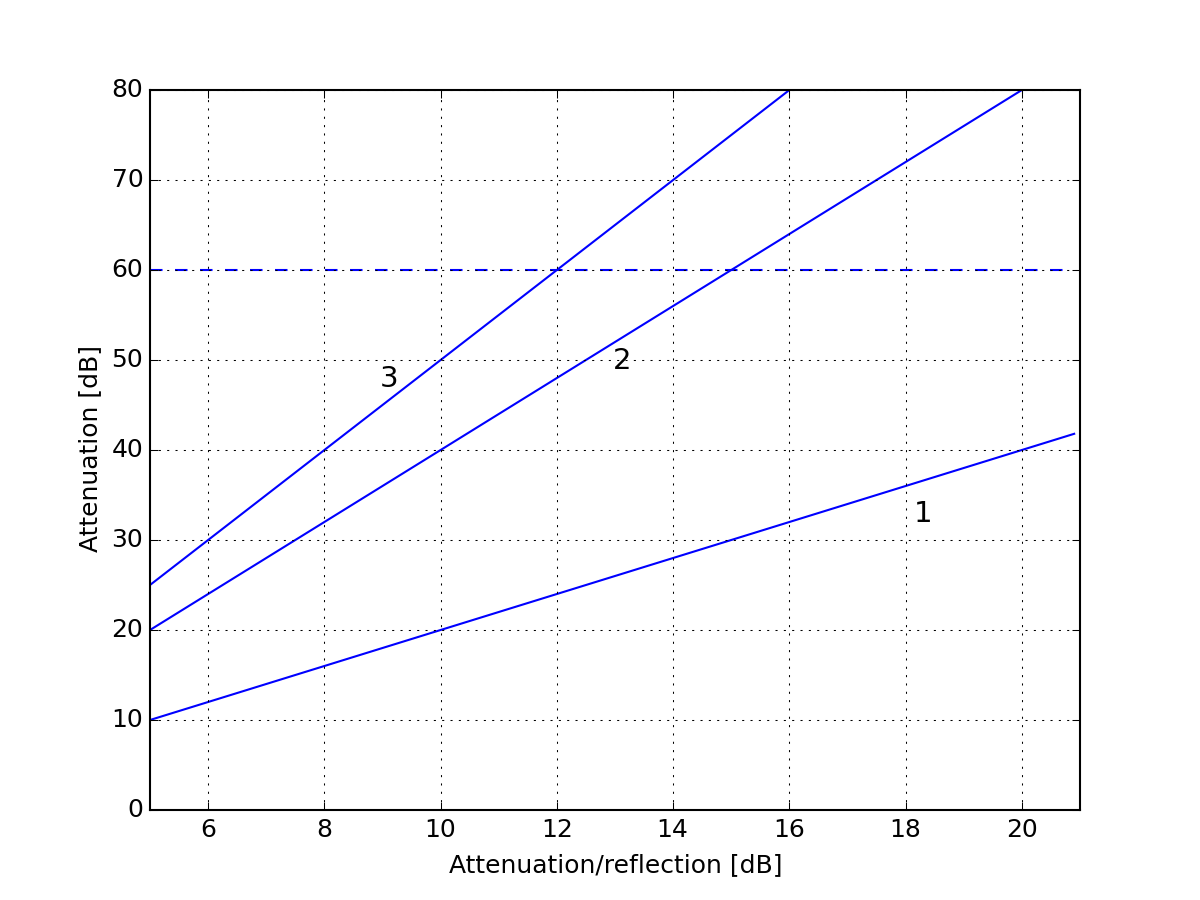
\includegraphics[width=1.0\textwidth]{bounces.png}
\caption{Overall attenuation for 1, 2 and 3 trips.}
\label{fig:bounces}
\end{figure}

One interpretation of the above is that we should have a diameter of 14-m or less and make sure we have 20 dB or more per "bounce".  

INCLUDE PLOT OF RELECTOMETRY TESTS

\section{Systematics}

\section{Sensitivity}
The equation for sensitivity has been described in previous works [REFS] and depends on many parameters
related to the instrumentation, the configuration, the location, the observing strategy, etc.  A useful form for 
the proposed compact configuration is Eq 27 in \citep{Parsonsetal2012} and reproduced here:
\begin{equation}
\centering
\label{eq:sensitivity}
\begin{split}
\Delta^2_N(k) \approx 60 \left[\frac{k}{0.1h\text{Mpc}^{-1}}\right]^\frac{5}{2}
                                         \left[\frac{6 \text{MHz}}{B}\right]^\frac{1}{2}
                                         \left[\frac{1}{\Delta\ln k}\right]^\frac{1}{2} \\
                        \times       \left[\frac{\Omega}{0.76\text{sr}}\right]
                                         \left[\frac{T_\text{sys}}{500 \text{K}}\right]^2
                                         \left[\frac{6 \text{hrs}}{t_\text{per\_day}}\right]^\frac{1}{2} \\
                        \times       \left[\frac{120\text{days}}{t_{\text{cam}}}\right]
                                         \left[\frac{32}{N_a}\right]
                                         \left[\frac{\text{10}^4f_o}{f}\right]  \text{mK}^2
\end{split}
\end{equation}
where $k$ is the magnitude of the $k$-mode, $B$ is the bandwidth, $\Delta\ln k$ is the log
of the binsize, $\Omega$ is the field-of-view, $T_{\text{sys}}$ is the system temperature, 
${t_\text{per\_day}}$ is the number of hours observed per day, $t_{\text{cam}}$ is the number of days
observed, $N_a$ is the number of antennas, and $f_o/f$ is the configuration metric for a 
redundant array as defined in \citep{Parsonsetal2012}.

Note that $\Delta^2_N(k)$ is the standard radiometric sensitivity equation, scaled by
the volume in $k$-space, normalized by the power spectrum Fourier coefficient, and
reduced by the number of independent samples in a given $k$-mode bin, which may have
both coherent and incoherent application.

Pulling out terms relating to diameter ($D_a$) and number, we can write Eq. \ref{eq:sensitivity} as
\begin{equation}
\label{eq:reducedSensitivity}
\Delta^2_N(k) \propto \frac{\Omega (f_o/f)}{N_a\sqrt{t_\text{per\_day}}} \propto \frac{(1/D_a^2)(1/\sqrt{N_a})}{N_a\sqrt{D_a}}
= D_a^{-\frac{5}{2}}N_a^{-\frac{3}{2}}
\end{equation}
where the dependencies on diameter and number have been substituted in, noting that the expressions for $f_o/f$ and 
$t_\text{per\_day}$were derived in Parsons et al where the baselines for the close-packed array are multiples of the diameter.

Letting the reduced sensitivity be $C = D_a^{-\frac{5}{2}}N_a^{-\frac{3}{2}}$ and scaling for canonical values of $D_a = 14$ m, $N_a = 331$ m, the needed number of antennas as a function of diameter (shown in Fig \ref{fig:Nsens}) is
\begin{equation}
\label{eq:Nmetric}
N_a = 26918 D_a^{-\frac{5}{3}}
\end{equation}

\begin{figure}[h]
\centering
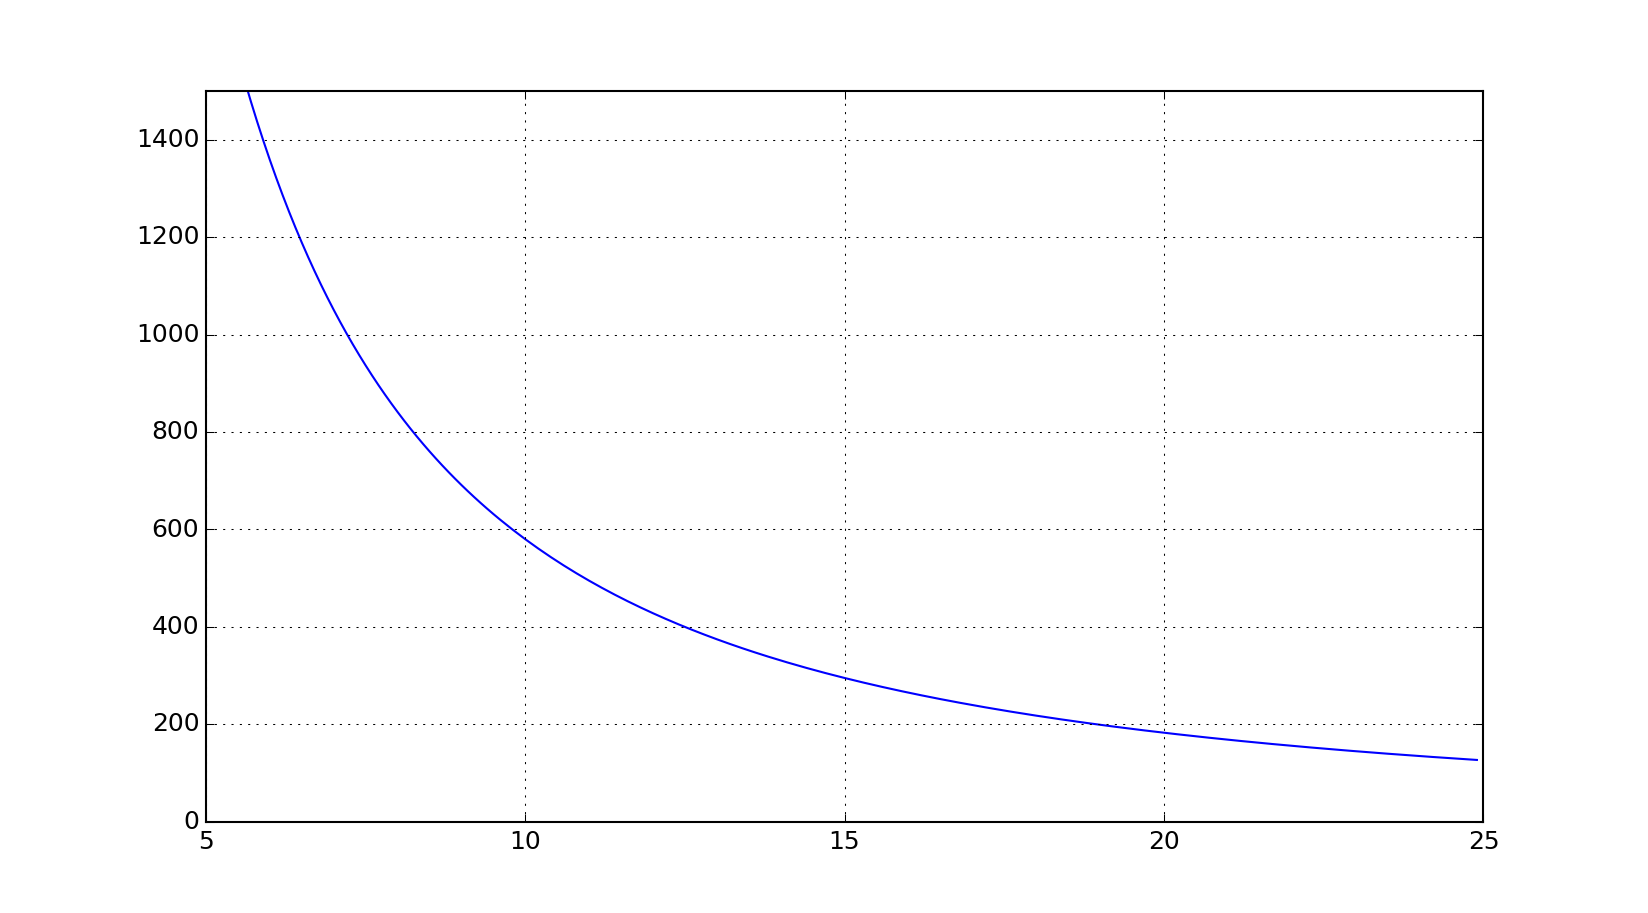
\includegraphics[width=0.8\textwidth]{Nsens.png}
\caption{Number of antennas at fixed sensitivity with reference of 331 14-m antennas}
\label{fig:Nsens}
\end{figure}

The sensitivity specification is to maximize performance per cost, which determines the element 
diameter ($D_a$) and the number of elements ($N_a$) subject to the constraints above.  One therefore 
needs a model of cost and performance as a function of $D_a$ and $N_a$.  Given a fairly mature element
and system design, a bottoms-up costing appropriate for element diameters from about 6-m to 30-m 
has been done for hex-numbers corresponding to element counts from 91 to 1141.  The costs here
are only those associated with delivering the array to that scope on-site, so excluding development and
science.  The results are shown in Fig. \ref{fig:normcost}.  At diameters greater than about 12-m the cost function
is relatively flat.

\begin{figure}[h]
\centering
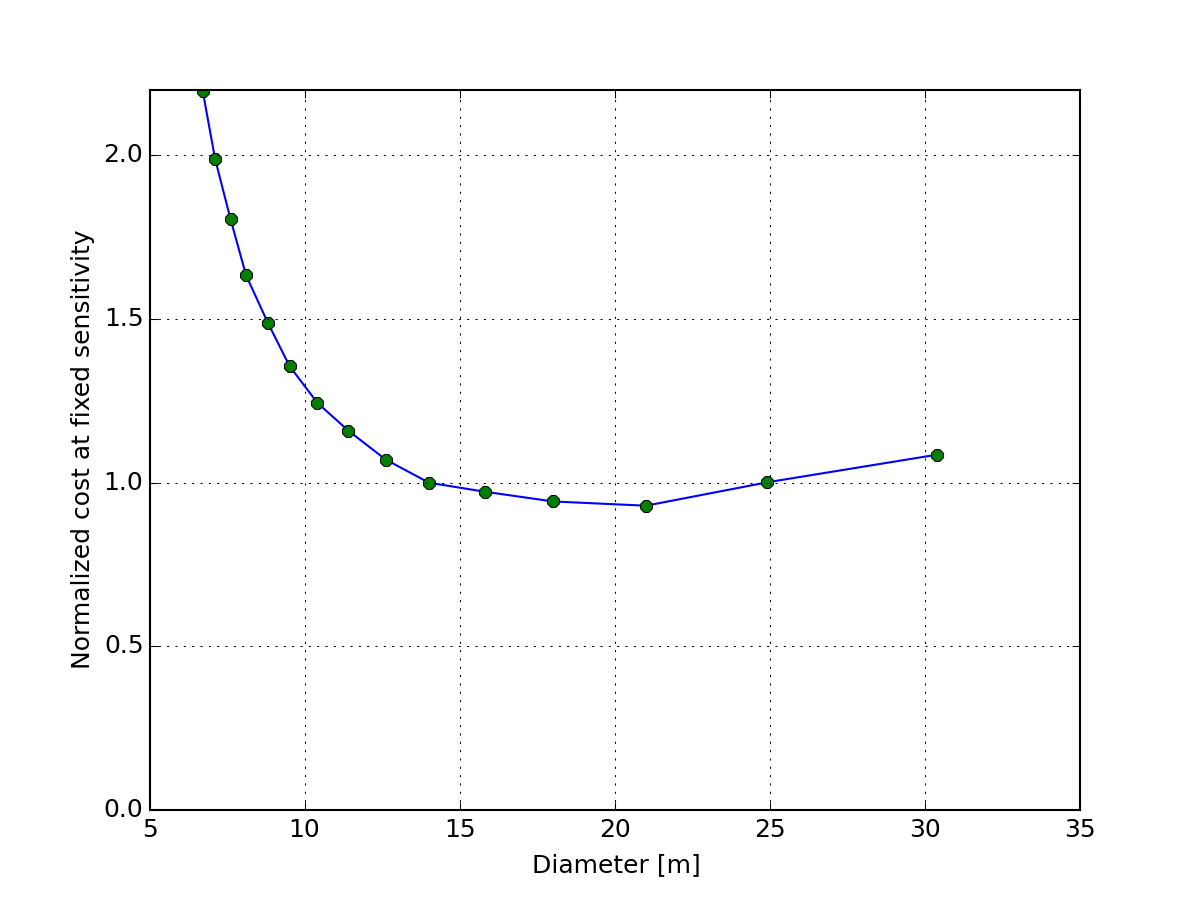
\includegraphics[width=0.8\textwidth]{normcostfunc.png}
\caption{Normalized cost at fixed sensitivity with reference of 331 14-m antennas}
\label{fig:normcost}
\end{figure}

\bibliographystyle{plainnat}
\bibliography{YOUR BIBLIOGRAPHY HERE}
\end{document}
